% $Id: christophe.tex,v 1.2 2001-06-11 07:50:49 geuzaine Exp $

\documentclass[a4]{seminar}

\usepackage{slides}

\renewcommand{\vec}[1]{\boldsymbol{#1}}
\newcommand{\mat}[1]{\mathbf{#1}}
\newcommand{\GradSymb}{\text{\bf grad}}
\newcommand{\CurlSymb}{\text{\bf curl}}
\newcommand{\DivSymb}{\text{\rm div}}
\newcommand{\pvec}[2]  {{#1}\times{#2}}
\newcommand{\psca}[2]  {{#1}\cdot{#2}}
\newcommand{\Curl}[1]  {\text{\CurlSymb}\,{#1}}\let\Rot\Curl
\newcommand{\Grad}[1]  {\text{\GradSymb}\,{#1}}
\newcommand{\Div}[1]   {\text{\DivSymb}\,{#1}}
\newcommand{\isur}[3][]{\langle#2,#3\rangle#1}
\newcommand{\ivol}[3][]{(#2,#3)#1}
\newcommand{\Ltwo}[2][]    {L^2#1(#2)}
\newcommand{\LLtwo}[2][]   {\boldsymbol{L}^2#1(#2)}
\newcommand{\Hone}[2][]    {H^1{#1}(#2)}
\newcommand{\Hcurl}[2][]   {\boldsymbol{H}#1(\CurlSymb;#2)}
\newcommand{\Hdiv}[2][]    {\boldsymbol{H}#1(\DivSymb;#2)}

\graphicspath{{.}{fig/}}

\begin{document}

\talk{CNRS Grenoble June 20, 2001}

% ---------------------------------------------------------------------------

\begin{slide}

\slidepagestyle{reduced}

\begin{center}
\bigtitle{Benefits of an open software environment for the modeling of
          coupled electromagnetic problems}\\
\bigskip\bigskip
\medtitle{Christophe Geuzaine}\\
\bigskip
\medtitle{Department of Electrical Engineering}\\
\medtitle{Montefiore Institute B28, Sart Tilman Campus}\\
\medtitle{University of Li�ge}\\
\medtitle{B-4000 Li�ge (BELGIUM)}
\end{center}

\end{slide}

% ---------------------------------------------------------------------------
\part{Introduction}
% ---------------------------------------------------------------------------

\chapter{Coupled electromagnetic problems?}

\begin{slide}

Maxwell's equations, coupled with...

\begin{slideitemize}
\item Electric and electronic \emph{circuits} (power electronic supplies)
\item \emph{Mechanical} phenomena (force calculation, magnetostriction,
piezoelectricity, noise and vibrations)
\item \emph{Thermal} phenomena (thermal losses, induction heating, dielectric heating)
\item \emph{Fluid} dynamics (charged particules, magnetohydrodynamics)
\end{slideitemize}

\end{slide}

% ---------------------------------------------------------------------------

\chapter{Computational methods?}

\begin{slide}

\begin{slideitemize}
\item \emph{Analytic} models are difficult/impossible to apply to complex/coupled problems
\item \emph{Performance} (both floating point and visualization) of low end PCs is
exploding
\item Basic \emph{theory} of classic numerical methods (finite differences, finite
volumes, finite elements, integral methods) is now well known, and future
developments don't change the fundamental principles anymore
\end{slideitemize}

\end{slide}

% ---------------------------------------------------------------------------

\chapter{Finite element method (FEM)}

\begin{slide}

\begin{slideitemize}
\item 1960s for mechanical problems (very large \emph{application range} since 1980s)
\item Strong \emph{mathematical foundations} (convergence, unicity)
\item Generalizations/reinterpretations (vanishing boundaries between finite
differences, finite elements and finite volumes, ...) call for a
\emph{single sofware implementation}
\end{slideitemize}

But FEM is not the magic/universal tool:
\begin{slideitemize}
\item Many conflicting/\emph{antinomic} issues (continuous
vs. discontinuous, conform vs. non conform meshes, implicit vs. explicit,
...)
\item Generality always has a price (i.e.\ \emph{efficiency} trade-off)
\end{slideitemize}

\end{slide}

\begin{slide}

Based on a double \emph{discretization}: ``replace'' the
\begin{slideitemize}
\item function spaces to which the field belong (e.g.\ $\Hone{\Omega}$,
$\Hcurl{\Omega}$, $\Hdiv{\Omega}$ and $\Ltwo{\Omega}$) by \emph{finite
dimensional function spaces}
\item domains on which these subspaces are defined by a union of elementary
geometrical elements of simple shapes (a ``\emph{mesh}'' or ``grid'')
\end{slideitemize}

\bigskip

\mybox{colbox}{\textwidth}{
\begin{center}
FEM\\ $\Updownarrow$\\ the finite dimensional subspaces are built so that
their bases are piecewise defined on the mesh
\end{center}
}

\end{slide}

\begin{slide}

One way to obtain a consistent Galerkin FEM formulation:
\begin{slideitemize}
\item Write a \emph{weak formulation} of the problem:

\begin{equation*}
\begin{cases}
L u = f \text{ in } \Omega \\
B u = g \text{ in } \Gamma 
\end{cases}
\Rightarrow\quad
\ivol[_\Omega]{u}{L^* v} - 
\ivol[_\Omega]{f}{v} + 
\int\limits_\Gamma Q_g(v) \, ds , 
\quad\forall v \in V(\Omega) 
\end{equation*}

% $L$ is a differential operator of order $n$ defined on $\Omega$
% 
% L^* is the adjoint of L:
%
% \ivol[_\Omega]{L u}{v} - \ivol[_\Omega]{u}{L^* v} = \int\limits_\Gamma Q(u,v) ds ,
%
% $Q$ is a bilinear function of $u$ and $v$ and in their derivatives up
% to the order $n-1$
%
% $Q_g$ is a linear form in $v$ which depends of $g$

\item Discretize with \emph{Whitney/Mixed} elements $w_i$:
\begin{equation*}
\bar{u}, \bar{v} \in W(\Omega) \subset V(\Omega), \quad
W(\Omega) = \text{span}\{w_i\} 
\end{equation*}

% \bar{u} = \sum_{i} u_i w_i 

\end{slideitemize}

\end{slide}

\begin{slide}

\begin{slideitemize}
\item ``\emph{nodal}'' elements for ``0-forms'' (\emph{continuous} scalar
fields like scalar potentials, temperature, pressure, ...)

\item ``\emph{edge}'' elements for ``1-forms'' (vector fields with
\emph{continuous tangential components} across material interfaces, like
electric and magnetic fields, magnetic vector potential, ...)

\item ``\emph{face}'' elements for ``2-forms'' (vector fields with
\emph{continuous normal components} across material interfaces, like
magnetic flux density, current density, ...)

\item ``\emph{volume}'' elements for ``3-forms'' (\emph{piecewise
continuous} scalar fields like charge density, heat source density, ...)

\end{slideitemize}

\end{slide}


\begin{slide}

The simplest example: magnetostatics

\begin{slideitemize}

\item Scalar potential:



\end{slideitemize}


\end{slide}

% ---------------------------------------------------------------------------

% $Id: getdp-basics.tex,v 1.1 2001-06-09 11:14:35 geuzaine Exp $

% ---------------------------------------------------------------------------

\chapter{}

\begin{slide}

\slidepagestyle{reduced}

\begin{center}
\bigtitle{A general software environment for the treatment of discrete problems}\\
\bigtitle{(GetDP)}\\
\bigskip\bigskip
\medtitle{Patrick Dular, Christophe Geuzaine}\\
\bigskip
\medtitle{Deptartment of Electrical Engineering}\\
\medtitle{Montefiore Institute B28, Sart Tilman Campus}\\
\medtitle{University of Li�ge}\\
\medtitle{B-4000 Li�ge (BELGIUM)}
\end{center}

\end{slide}

% ---------------------------------------------------------------------------
\part{GetDP}
% ---------------------------------------------------------------------------

\chapter{An environment open to various couplings}

\begin{slide}

Any coupling between 
\begin{slideitemize}
\item \emph{Physical} problems (electromagnetic, thermal, mechanical, ...)
\item \emph{Numerical} methods (finite element methods, integral methods, ...)
\item \emph{Geometries} (1D, 2D, 2D axi, 3D)
\item \emph{Time} states (static, harmonic, transient)
\end{slideitemize}

How?
\begin{slideitemize}
\item Clear \emph{mathematical} definitions/structure
\item Directly transcribed into 10 interdependent \emph{objects}
\end{slideitemize}

\end{slide}

% ---------------------------------------------------------------------------

\chapter{Definition of discrete problems}

\begin{slide}

\begin{slideitemize}
\item Copy of formal mathematical expression of problems 
\item ASCII \emph{Text} file (``\code{.pro} file'')
\end{slideitemize}

\begin{center}
\scalebox{0.54}{\begin{picture}(0,0)%
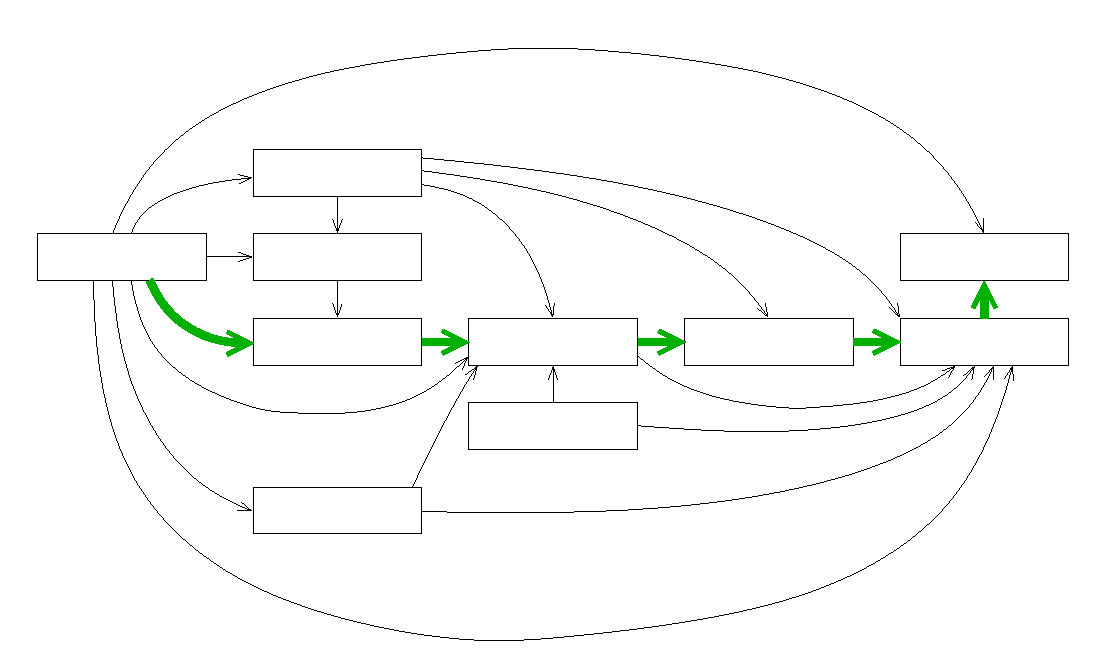
\includegraphics{getdp-struct}%
\end{picture}%
\setlength{\unitlength}{3947sp}%
%
\begingroup\makeatletter\ifx\SetFigFont\undefined%
\gdef\SetFigFont#1#2#3#4#5{%
  \reset@font\fontsize{#1}{#2pt}%
  \fontfamily{#3}\fontseries{#4}\fontshape{#5}%
  \selectfont}%
\fi\endgroup%
\begin{picture}(8552,4992)(300,-6402)
\put(1126,-3361){\makebox(0,0)[b]{\smash{\SetFigFont{10}{12.0}{\rmdefault}{\mddefault}{\updefault}{\color[rgb]{0,0,0}\code{Group}}%
}}}
\put(2851,-2686){\makebox(0,0)[b]{\smash{\SetFigFont{10}{12.0}{\rmdefault}{\mddefault}{\updefault}{\color[rgb]{0,0,0}\code{Function}}%
}}}
\put(2851,-3361){\makebox(0,0)[b]{\smash{\SetFigFont{10}{12.0}{\rmdefault}{\mddefault}{\updefault}{\color[rgb]{0,0,0}\code{Constraint}}%
}}}
\put(2851,-4036){\makebox(0,0)[b]{\smash{\SetFigFont{10}{12.0}{\rmdefault}{\mddefault}{\updefault}{\color[rgb]{0,0,0}\code{FunctionSpace}}%
}}}
\put(2851,-5386){\makebox(0,0)[b]{\smash{\SetFigFont{10}{12.0}{\rmdefault}{\mddefault}{\updefault}{\color[rgb]{0,0,0}\code{Jacobian}}%
}}}
\put(4576,-4711){\makebox(0,0)[b]{\smash{\SetFigFont{10}{12.0}{\rmdefault}{\mddefault}{\updefault}{\color[rgb]{0,0,0}\code{Integration}}%
}}}
\put(4576,-4036){\makebox(0,0)[b]{\smash{\SetFigFont{10}{12.0}{\rmdefault}{\mddefault}{\updefault}{\color[rgb]{0,0,0}\code{Formulation}}%
}}}
\put(6301,-4036){\makebox(0,0)[b]{\smash{\SetFigFont{10}{12.0}{\rmdefault}{\mddefault}{\updefault}{\color[rgb]{0,0,0}\code{Resolution}}%
}}}
\put(8026,-3361){\makebox(0,0)[b]{\smash{\SetFigFont{10}{12.0}{\rmdefault}{\mddefault}{\updefault}{\color[rgb]{0,0,0}\code{PostOperation}}%
}}}
\put(8026,-4036){\makebox(0,0)[b]{\smash{\SetFigFont{10}{12.0}{\rmdefault}{\mddefault}{\updefault}{\color[rgb]{0,0,0}\code{PostProcessing}}%
}}}
\end{picture}
}
\end{center}

\end{slide}

\begin{slide}

\begin{center}
Particular data of a problem\\
\medskip
\scalebox{0.54}{\begin{picture}(0,0)%
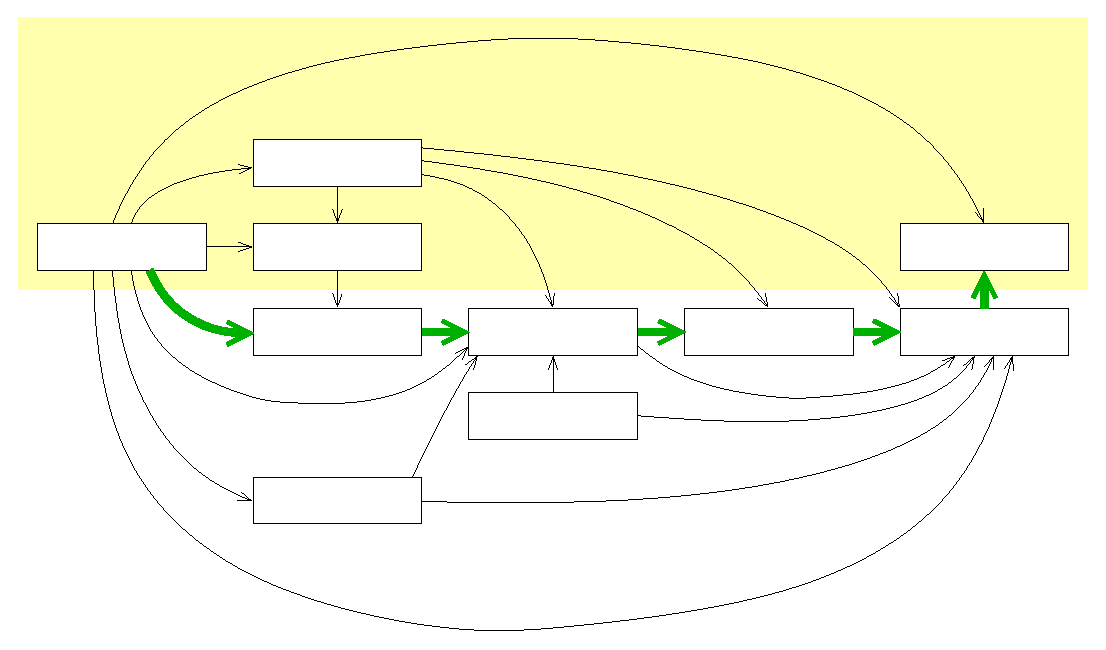
\includegraphics{getdp-struct-box}%
\end{picture}%
\setlength{\unitlength}{3947sp}%
%
\begingroup\makeatletter\ifx\SetFigFont\undefined%
\gdef\SetFigFont#1#2#3#4#5{%
  \reset@font\fontsize{#1}{#2pt}%
  \fontfamily{#3}\fontseries{#4}\fontshape{#5}%
  \selectfont}%
\fi\endgroup%
\begin{picture}(8552,4917)(300,-6402)
\put(1126,-3361){\makebox(0,0)[b]{\smash{\SetFigFont{10}{12.0}{\rmdefault}{\mddefault}{\updefault}{\color[rgb]{0,0,0}\code{Group}}%
}}}
\put(2851,-2686){\makebox(0,0)[b]{\smash{\SetFigFont{10}{12.0}{\rmdefault}{\mddefault}{\updefault}{\color[rgb]{0,0,0}\code{Function}}%
}}}
\put(2851,-3361){\makebox(0,0)[b]{\smash{\SetFigFont{10}{12.0}{\rmdefault}{\mddefault}{\updefault}{\color[rgb]{0,0,0}\code{Constraint}}%
}}}
\put(2851,-4036){\makebox(0,0)[b]{\smash{\SetFigFont{10}{12.0}{\rmdefault}{\mddefault}{\updefault}{\color[rgb]{0,0,0}\code{FunctionSpace}}%
}}}
\put(2851,-5386){\makebox(0,0)[b]{\smash{\SetFigFont{10}{12.0}{\rmdefault}{\mddefault}{\updefault}{\color[rgb]{0,0,0}\code{Jacobian}}%
}}}
\put(4576,-4711){\makebox(0,0)[b]{\smash{\SetFigFont{10}{12.0}{\rmdefault}{\mddefault}{\updefault}{\color[rgb]{0,0,0}\code{Integration}}%
}}}
\put(4576,-4036){\makebox(0,0)[b]{\smash{\SetFigFont{10}{12.0}{\rmdefault}{\mddefault}{\updefault}{\color[rgb]{0,0,0}\code{Formulation}}%
}}}
\put(6301,-4036){\makebox(0,0)[b]{\smash{\SetFigFont{10}{12.0}{\rmdefault}{\mddefault}{\updefault}{\color[rgb]{0,0,0}\code{Resolution}}%
}}}
\put(8026,-3361){\makebox(0,0)[b]{\smash{\SetFigFont{10}{12.0}{\rmdefault}{\mddefault}{\updefault}{\color[rgb]{0,0,0}\code{PostOperation}}%
}}}
\put(8026,-4036){\makebox(0,0)[b]{\smash{\SetFigFont{10}{12.0}{\rmdefault}{\mddefault}{\updefault}{\color[rgb]{0,0,0}\code{PostProcessing}}%
}}}
\end{picture}
}\\
\medskip
Method of resolution (``black box'')
\end{center}

\end{slide}

% ---------------------------------------------------------------------------

\background{7\semcm}{4.2\semcm}{\scalebox{0.3}{\begin{picture}(0,0)%
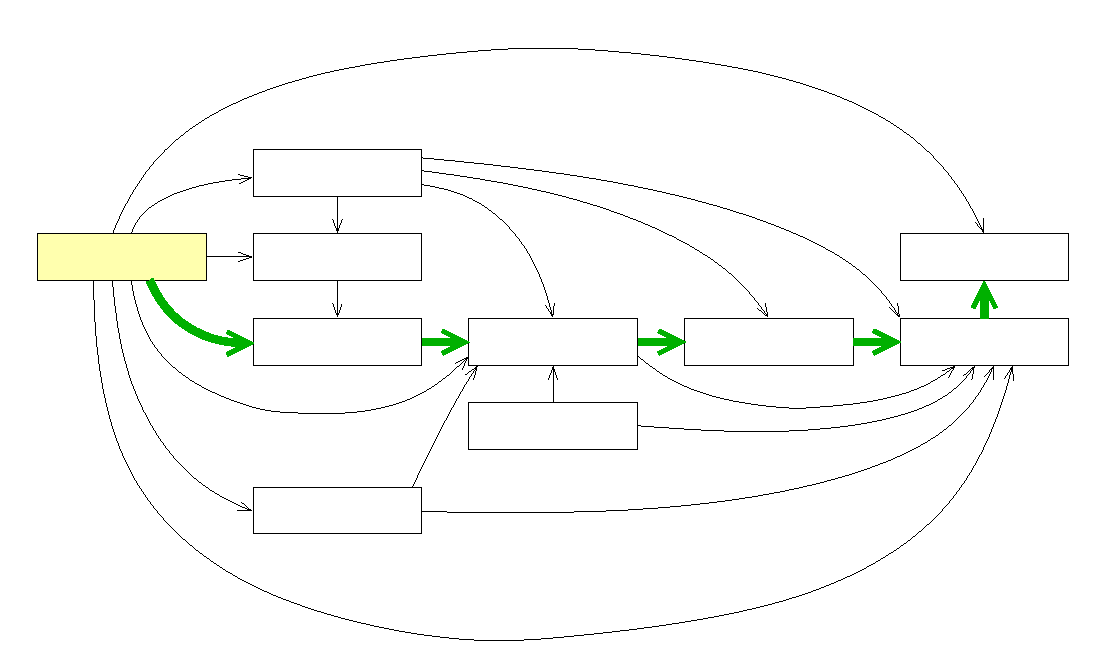
\includegraphics{getdp-struct-group}%
\end{picture}%
\setlength{\unitlength}{3947sp}%
%
\begingroup\makeatletter\ifx\SetFigFont\undefined%
\gdef\SetFigFont#1#2#3#4#5{%
  \reset@font\fontsize{#1}{#2pt}%
  \fontfamily{#3}\fontseries{#4}\fontshape{#5}%
  \selectfont}%
\fi\endgroup%
\begin{picture}(8274,4765)(439,-6402)
\put(1126,-3361){\makebox(0,0)[b]{\smash{\SetFigFont{10}{12.0}{\rmdefault}{\mddefault}{\updefault}{\color[rgb]{0,0,0}\code{Group}}%
}}}
\put(2851,-2686){\makebox(0,0)[b]{\smash{\SetFigFont{10}{12.0}{\rmdefault}{\mddefault}{\updefault}{\color[rgb]{0,0,0}\code{Function}}%
}}}
\put(2851,-3361){\makebox(0,0)[b]{\smash{\SetFigFont{10}{12.0}{\rmdefault}{\mddefault}{\updefault}{\color[rgb]{0,0,0}\code{Constraint}}%
}}}
\put(2851,-4036){\makebox(0,0)[b]{\smash{\SetFigFont{10}{12.0}{\rmdefault}{\mddefault}{\updefault}{\color[rgb]{0,0,0}\code{FunctionSpace}}%
}}}
\put(2851,-5386){\makebox(0,0)[b]{\smash{\SetFigFont{10}{12.0}{\rmdefault}{\mddefault}{\updefault}{\color[rgb]{0,0,0}\code{Jacobian}}%
}}}
\put(4576,-4711){\makebox(0,0)[b]{\smash{\SetFigFont{10}{12.0}{\rmdefault}{\mddefault}{\updefault}{\color[rgb]{0,0,0}\code{Integration}}%
}}}
\put(4576,-4036){\makebox(0,0)[b]{\smash{\SetFigFont{10}{12.0}{\rmdefault}{\mddefault}{\updefault}{\color[rgb]{0,0,0}\code{Formulation}}%
}}}
\put(6301,-4036){\makebox(0,0)[b]{\smash{\SetFigFont{10}{12.0}{\rmdefault}{\mddefault}{\updefault}{\color[rgb]{0,0,0}\code{Resolution}}%
}}}
\put(8026,-3361){\makebox(0,0)[b]{\smash{\SetFigFont{10}{12.0}{\rmdefault}{\mddefault}{\updefault}{\color[rgb]{0,0,0}\code{PostOperation}}%
}}}
\put(8026,-4036){\makebox(0,0)[b]{\smash{\SetFigFont{10}{12.0}{\rmdefault}{\mddefault}{\updefault}{\color[rgb]{0,0,0}\code{PostProcessing}}%
}}}
\end{picture}
}}

\chapter{\code{Group}: defining topological entities}

\begin{slide}

\mybox{colbox}{11\semcm}{
  \begin{slideitemize}
  \item Regions
  \item Functions on Regions (nodes, edges, edges of tree, ...)
  \end{slideitemize}
}

Example:

\begin{syntax}
Air = Region[1]; Core = Region[2];
    = ;
\end{syntax}



\end{slide}

% ---------------------------------------------------------------------------

\background{7\semcm}{4.2\semcm}{\scalebox{0.3}{\begin{picture}(0,0)%
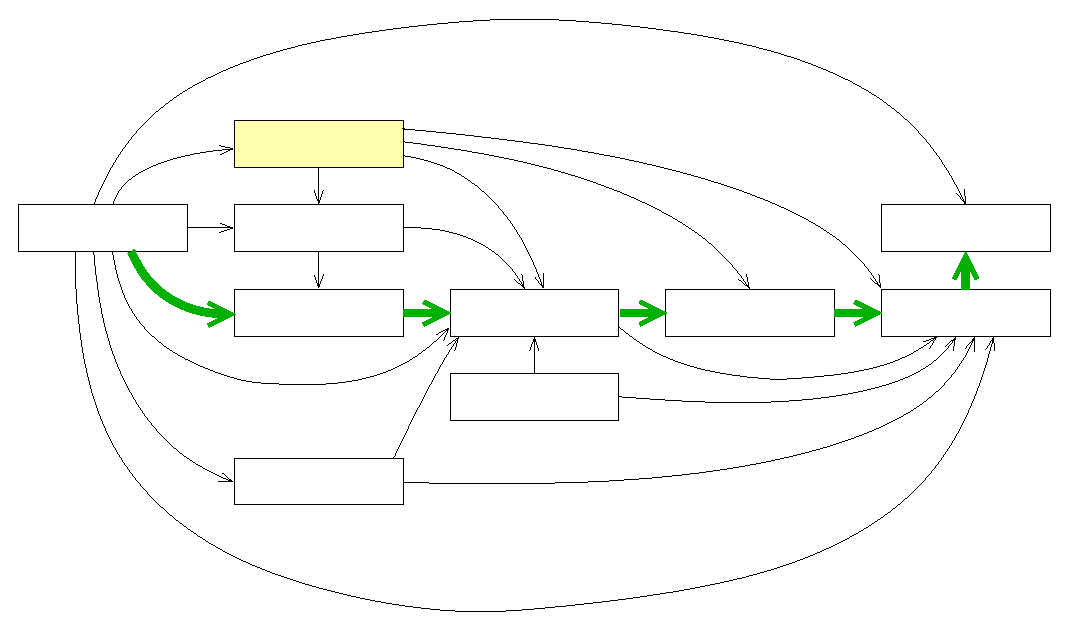
\includegraphics{getdp-struct-function}%
\end{picture}%
\setlength{\unitlength}{3947sp}%
%
\begingroup\makeatletter\ifx\SetFigFont\undefined%
\gdef\SetFigFont#1#2#3#4#5{%
  \reset@font\fontsize{#1}{#2pt}%
  \fontfamily{#3}\fontseries{#4}\fontshape{#5}%
  \selectfont}%
\fi\endgroup%
\begin{picture}(8274,4765)(439,-6402)
\put(1126,-3361){\makebox(0,0)[b]{\smash{\SetFigFont{10}{12.0}{\rmdefault}{\mddefault}{\updefault}{\color[rgb]{0,0,0}\code{Group}}%
}}}
\put(2851,-2686){\makebox(0,0)[b]{\smash{\SetFigFont{10}{12.0}{\rmdefault}{\mddefault}{\updefault}{\color[rgb]{0,0,0}\code{Function}}%
}}}
\put(2851,-3361){\makebox(0,0)[b]{\smash{\SetFigFont{10}{12.0}{\rmdefault}{\mddefault}{\updefault}{\color[rgb]{0,0,0}\code{Constraint}}%
}}}
\put(2851,-4036){\makebox(0,0)[b]{\smash{\SetFigFont{10}{12.0}{\rmdefault}{\mddefault}{\updefault}{\color[rgb]{0,0,0}\code{FunctionSpace}}%
}}}
\put(2851,-5386){\makebox(0,0)[b]{\smash{\SetFigFont{10}{12.0}{\rmdefault}{\mddefault}{\updefault}{\color[rgb]{0,0,0}\code{Jacobian}}%
}}}
\put(4576,-4711){\makebox(0,0)[b]{\smash{\SetFigFont{10}{12.0}{\rmdefault}{\mddefault}{\updefault}{\color[rgb]{0,0,0}\code{Integration}}%
}}}
\put(4576,-4036){\makebox(0,0)[b]{\smash{\SetFigFont{10}{12.0}{\rmdefault}{\mddefault}{\updefault}{\color[rgb]{0,0,0}\code{Formulation}}%
}}}
\put(6301,-4036){\makebox(0,0)[b]{\smash{\SetFigFont{10}{12.0}{\rmdefault}{\mddefault}{\updefault}{\color[rgb]{0,0,0}\code{Resolution}}%
}}}
\put(8026,-3361){\makebox(0,0)[b]{\smash{\SetFigFont{10}{12.0}{\rmdefault}{\mddefault}{\updefault}{\color[rgb]{0,0,0}\code{PostOperation}}%
}}}
\put(8026,-4036){\makebox(0,0)[b]{\smash{\SetFigFont{10}{12.0}{\rmdefault}{\mddefault}{\updefault}{\color[rgb]{0,0,0}\code{PostProcessing}}%
}}}
\end{picture}
}}

\chapter{\code{Function}: defining expressions}

\begin{slide}

\mybox{colbox}{11\semcm}{
  \begin{slideitemize}
  \item Physical characteristics
  \item Time functions
  \item Various other functions (natural contraints, ...)
  \end{slideitemize}
}

Example:


\end{slide}

% ---------------------------------------------------------------------------

\background{7\semcm}{4.2\semcm}{\scalebox{0.3}{\begin{picture}(0,0)%
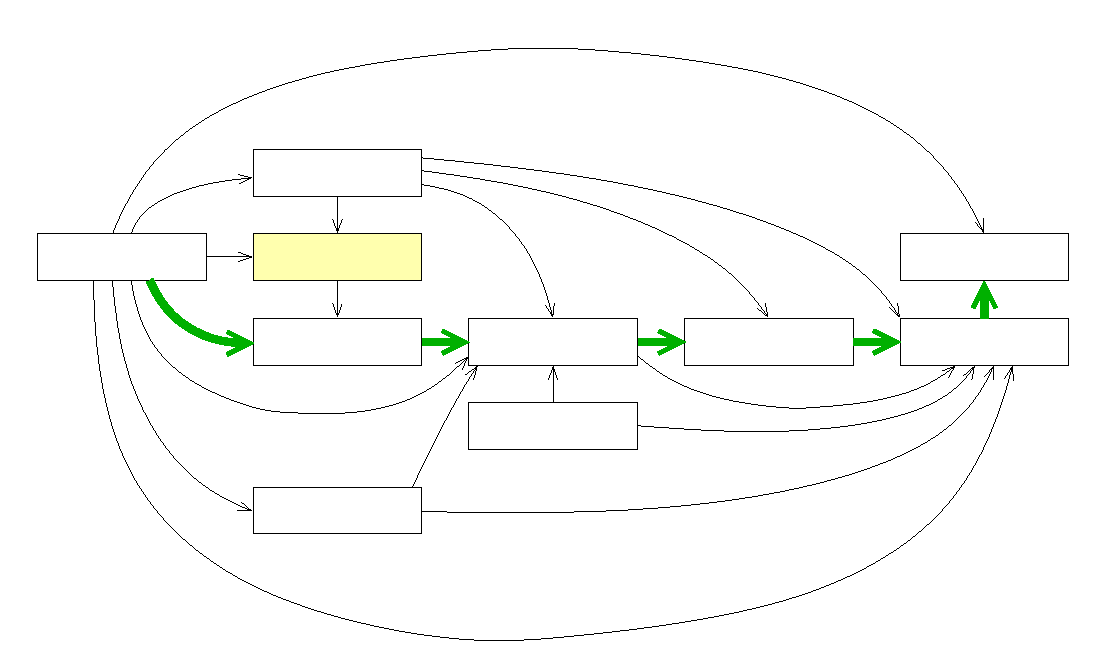
\includegraphics{getdp-struct-constraint}%
\end{picture}%
\setlength{\unitlength}{3947sp}%
%
\begingroup\makeatletter\ifx\SetFigFont\undefined%
\gdef\SetFigFont#1#2#3#4#5{%
  \reset@font\fontsize{#1}{#2pt}%
  \fontfamily{#3}\fontseries{#4}\fontshape{#5}%
  \selectfont}%
\fi\endgroup%
\begin{picture}(8274,4765)(439,-6402)
\put(1126,-3361){\makebox(0,0)[b]{\smash{\SetFigFont{10}{12.0}{\rmdefault}{\mddefault}{\updefault}{\color[rgb]{0,0,0}\code{Group}}%
}}}
\put(2851,-2686){\makebox(0,0)[b]{\smash{\SetFigFont{10}{12.0}{\rmdefault}{\mddefault}{\updefault}{\color[rgb]{0,0,0}\code{Function}}%
}}}
\put(2851,-3361){\makebox(0,0)[b]{\smash{\SetFigFont{10}{12.0}{\rmdefault}{\mddefault}{\updefault}{\color[rgb]{0,0,0}\code{Constraint}}%
}}}
\put(2851,-4036){\makebox(0,0)[b]{\smash{\SetFigFont{10}{12.0}{\rmdefault}{\mddefault}{\updefault}{\color[rgb]{0,0,0}\code{FunctionSpace}}%
}}}
\put(2851,-5386){\makebox(0,0)[b]{\smash{\SetFigFont{10}{12.0}{\rmdefault}{\mddefault}{\updefault}{\color[rgb]{0,0,0}\code{Jacobian}}%
}}}
\put(4576,-4711){\makebox(0,0)[b]{\smash{\SetFigFont{10}{12.0}{\rmdefault}{\mddefault}{\updefault}{\color[rgb]{0,0,0}\code{Integration}}%
}}}
\put(4576,-4036){\makebox(0,0)[b]{\smash{\SetFigFont{10}{12.0}{\rmdefault}{\mddefault}{\updefault}{\color[rgb]{0,0,0}\code{Formulation}}%
}}}
\put(6301,-4036){\makebox(0,0)[b]{\smash{\SetFigFont{10}{12.0}{\rmdefault}{\mddefault}{\updefault}{\color[rgb]{0,0,0}\code{Resolution}}%
}}}
\put(8026,-3361){\makebox(0,0)[b]{\smash{\SetFigFont{10}{12.0}{\rmdefault}{\mddefault}{\updefault}{\color[rgb]{0,0,0}\code{PostOperation}}%
}}}
\put(8026,-4036){\makebox(0,0)[b]{\smash{\SetFigFont{10}{12.0}{\rmdefault}{\mddefault}{\updefault}{\color[rgb]{0,0,0}\code{PostProcessing}}%
}}}
\end{picture}
}}

\chapter{\code{Constraint}: specifying constraints}

\begin{slide}

\mybox{colbox}{11\semcm}{
  \begin{slideitemize}
  \item Boundary conditions (classical, connection)
  \item Initial conditions
  \item Topology of circuits with lumped elements
  \item Other constraints (on local and global quantities)
  \end{slideitemize}
}

Example:


\end{slide}

% ---------------------------------------------------------------------------

\background{7\semcm}{4.2\semcm}{\scalebox{0.3}{\begin{picture}(0,0)%
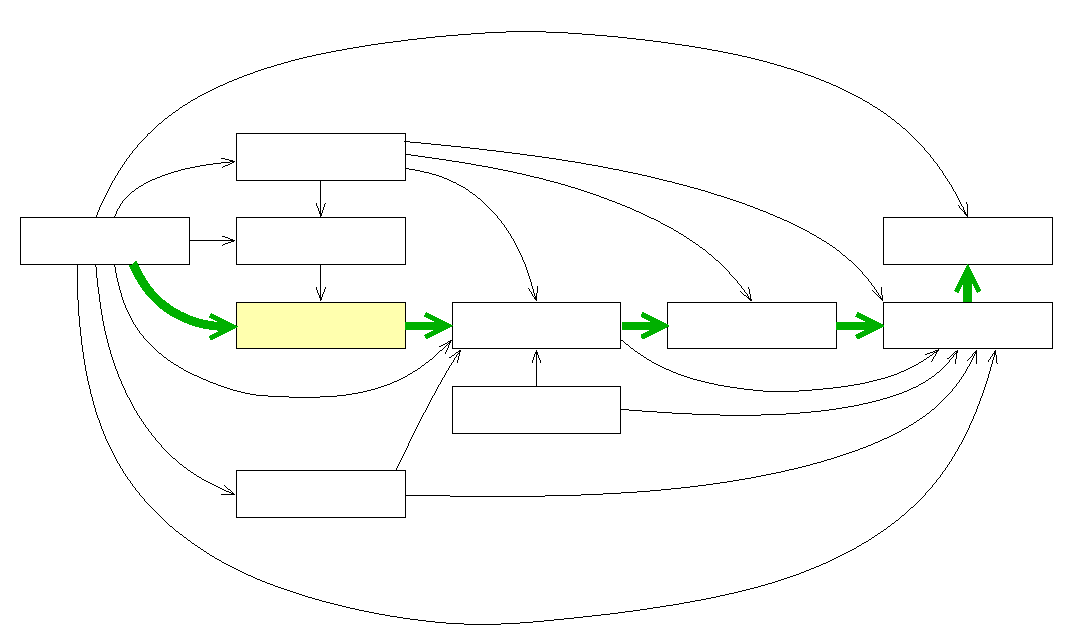
\includegraphics{getdp-struct-functionspace}%
\end{picture}%
\setlength{\unitlength}{3947sp}%
%
\begingroup\makeatletter\ifx\SetFigFont\undefined%
\gdef\SetFigFont#1#2#3#4#5{%
  \reset@font\fontsize{#1}{#2pt}%
  \fontfamily{#3}\fontseries{#4}\fontshape{#5}%
  \selectfont}%
\fi\endgroup%
\begin{picture}(8552,4992)(300,-6402)
\put(1126,-3361){\makebox(0,0)[b]{\smash{\SetFigFont{10}{12.0}{\rmdefault}{\mddefault}{\updefault}{\color[rgb]{0,0,0}\code{Group}}%
}}}
\put(2851,-2686){\makebox(0,0)[b]{\smash{\SetFigFont{10}{12.0}{\rmdefault}{\mddefault}{\updefault}{\color[rgb]{0,0,0}\code{Function}}%
}}}
\put(2851,-3361){\makebox(0,0)[b]{\smash{\SetFigFont{10}{12.0}{\rmdefault}{\mddefault}{\updefault}{\color[rgb]{0,0,0}\code{Constraint}}%
}}}
\put(2851,-4036){\makebox(0,0)[b]{\smash{\SetFigFont{10}{12.0}{\rmdefault}{\mddefault}{\updefault}{\color[rgb]{0,0,0}\code{FunctionSpace}}%
}}}
\put(2851,-5386){\makebox(0,0)[b]{\smash{\SetFigFont{10}{12.0}{\rmdefault}{\mddefault}{\updefault}{\color[rgb]{0,0,0}\code{Jacobian}}%
}}}
\put(4576,-4711){\makebox(0,0)[b]{\smash{\SetFigFont{10}{12.0}{\rmdefault}{\mddefault}{\updefault}{\color[rgb]{0,0,0}\code{Integration}}%
}}}
\put(4576,-4036){\makebox(0,0)[b]{\smash{\SetFigFont{10}{12.0}{\rmdefault}{\mddefault}{\updefault}{\color[rgb]{0,0,0}\code{Formulation}}%
}}}
\put(6301,-4036){\makebox(0,0)[b]{\smash{\SetFigFont{10}{12.0}{\rmdefault}{\mddefault}{\updefault}{\color[rgb]{0,0,0}\code{Resolution}}%
}}}
\put(8026,-3361){\makebox(0,0)[b]{\smash{\SetFigFont{10}{12.0}{\rmdefault}{\mddefault}{\updefault}{\color[rgb]{0,0,0}\code{PostOperation}}%
}}}
\put(8026,-4036){\makebox(0,0)[b]{\smash{\SetFigFont{10}{12.0}{\rmdefault}{\mddefault}{\updefault}{\color[rgb]{0,0,0}\code{PostProcessing}}%
}}}
\end{picture}
}}

\chapter{\code{FunctionSpace}: building function spaces}

\begin{slide}



Example:


\end{slide}

% ---------------------------------------------------------------------------

\background{7\semcm}{4.2\semcm}{\scalebox{0.3}{\begin{picture}(0,0)%
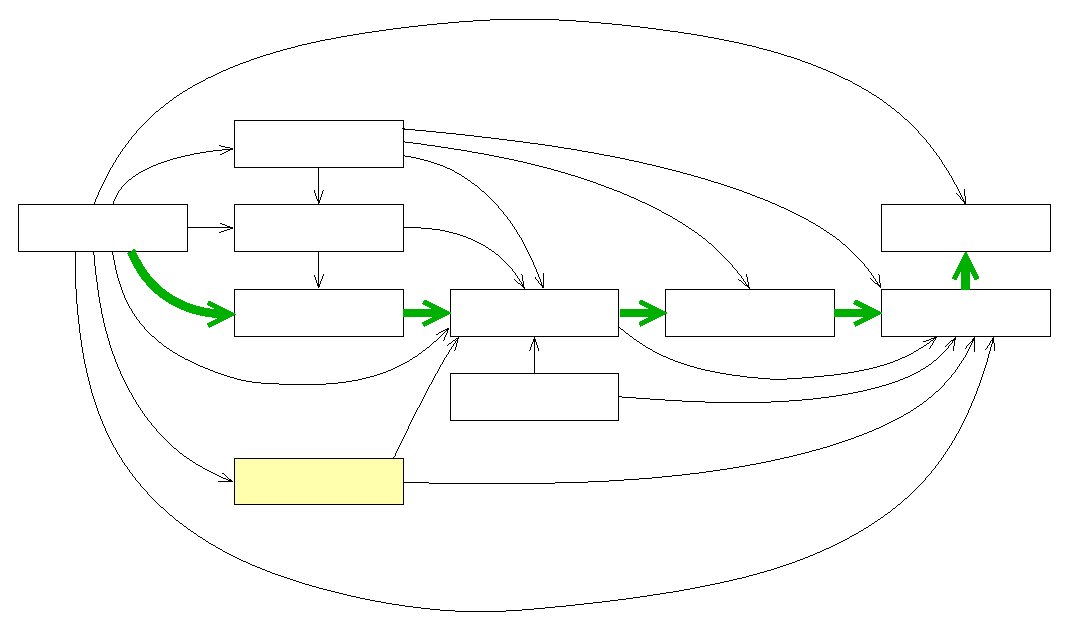
\includegraphics{getdp-struct-jacobian}%
\end{picture}%
\setlength{\unitlength}{3947sp}%
%
\begingroup\makeatletter\ifx\SetFigFont\undefined%
\gdef\SetFigFont#1#2#3#4#5{%
  \reset@font\fontsize{#1}{#2pt}%
  \fontfamily{#3}\fontseries{#4}\fontshape{#5}%
  \selectfont}%
\fi\endgroup%
\begin{picture}(8274,4765)(439,-6402)
\put(1126,-3361){\makebox(0,0)[b]{\smash{\SetFigFont{10}{12.0}{\rmdefault}{\mddefault}{\updefault}{\color[rgb]{0,0,0}\code{Group}}%
}}}
\put(2851,-2686){\makebox(0,0)[b]{\smash{\SetFigFont{10}{12.0}{\rmdefault}{\mddefault}{\updefault}{\color[rgb]{0,0,0}\code{Function}}%
}}}
\put(2851,-3361){\makebox(0,0)[b]{\smash{\SetFigFont{10}{12.0}{\rmdefault}{\mddefault}{\updefault}{\color[rgb]{0,0,0}\code{Constraint}}%
}}}
\put(2851,-4036){\makebox(0,0)[b]{\smash{\SetFigFont{10}{12.0}{\rmdefault}{\mddefault}{\updefault}{\color[rgb]{0,0,0}\code{FunctionSpace}}%
}}}
\put(2851,-5386){\makebox(0,0)[b]{\smash{\SetFigFont{10}{12.0}{\rmdefault}{\mddefault}{\updefault}{\color[rgb]{0,0,0}\code{Jacobian}}%
}}}
\put(4576,-4711){\makebox(0,0)[b]{\smash{\SetFigFont{10}{12.0}{\rmdefault}{\mddefault}{\updefault}{\color[rgb]{0,0,0}\code{Integration}}%
}}}
\put(4576,-4036){\makebox(0,0)[b]{\smash{\SetFigFont{10}{12.0}{\rmdefault}{\mddefault}{\updefault}{\color[rgb]{0,0,0}\code{Formulation}}%
}}}
\put(6301,-4036){\makebox(0,0)[b]{\smash{\SetFigFont{10}{12.0}{\rmdefault}{\mddefault}{\updefault}{\color[rgb]{0,0,0}\code{Resolution}}%
}}}
\put(8026,-3361){\makebox(0,0)[b]{\smash{\SetFigFont{10}{12.0}{\rmdefault}{\mddefault}{\updefault}{\color[rgb]{0,0,0}\code{PostOperation}}%
}}}
\put(8026,-4036){\makebox(0,0)[b]{\smash{\SetFigFont{10}{12.0}{\rmdefault}{\mddefault}{\updefault}{\color[rgb]{0,0,0}\code{PostProcessing}}%
}}}
\end{picture}
}}

\chapter{\code{Jacobian}: defining jacobian methods}

\begin{slide}


Example:


\end{slide}

% ---------------------------------------------------------------------------

\background{7\semcm}{4.2\semcm}{\scalebox{0.3}{\begin{picture}(0,0)%
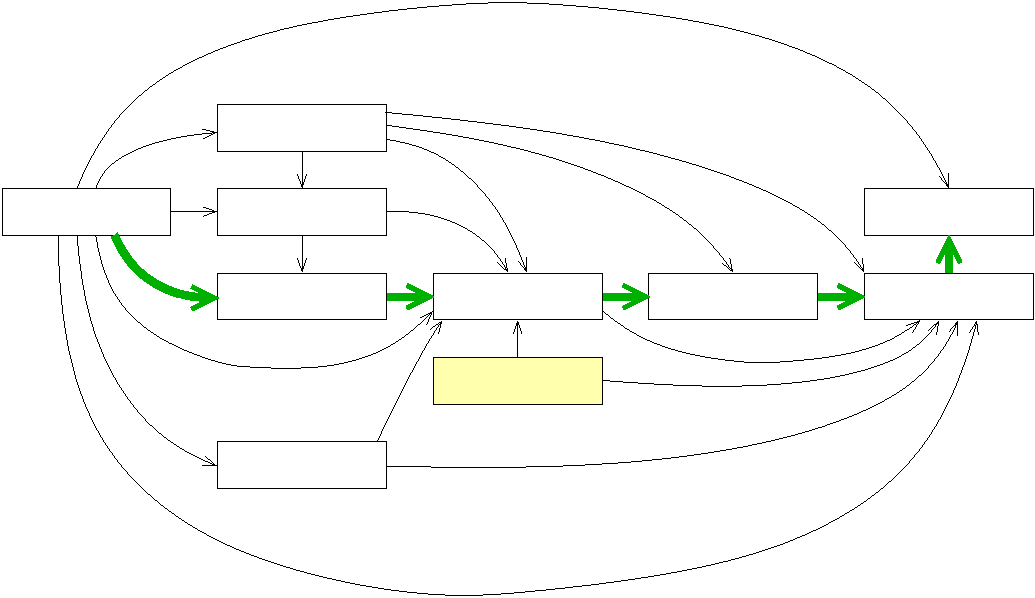
\includegraphics{getdp-struct-integration}%
\end{picture}%
\setlength{\unitlength}{3947sp}%
%
\begingroup\makeatletter\ifx\SetFigFont\undefined%
\gdef\SetFigFont#1#2#3#4#5{%
  \reset@font\fontsize{#1}{#2pt}%
  \fontfamily{#3}\fontseries{#4}\fontshape{#5}%
  \selectfont}%
\fi\endgroup%
\begin{picture}(8552,4992)(300,-6402)
\put(1126,-3361){\makebox(0,0)[b]{\smash{\SetFigFont{10}{12.0}{\rmdefault}{\mddefault}{\updefault}{\color[rgb]{0,0,0}\code{Group}}%
}}}
\put(2851,-2686){\makebox(0,0)[b]{\smash{\SetFigFont{10}{12.0}{\rmdefault}{\mddefault}{\updefault}{\color[rgb]{0,0,0}\code{Function}}%
}}}
\put(2851,-3361){\makebox(0,0)[b]{\smash{\SetFigFont{10}{12.0}{\rmdefault}{\mddefault}{\updefault}{\color[rgb]{0,0,0}\code{Constraint}}%
}}}
\put(2851,-4036){\makebox(0,0)[b]{\smash{\SetFigFont{10}{12.0}{\rmdefault}{\mddefault}{\updefault}{\color[rgb]{0,0,0}\code{FunctionSpace}}%
}}}
\put(2851,-5386){\makebox(0,0)[b]{\smash{\SetFigFont{10}{12.0}{\rmdefault}{\mddefault}{\updefault}{\color[rgb]{0,0,0}\code{Jacobian}}%
}}}
\put(4576,-4711){\makebox(0,0)[b]{\smash{\SetFigFont{10}{12.0}{\rmdefault}{\mddefault}{\updefault}{\color[rgb]{0,0,0}\code{Integration}}%
}}}
\put(4576,-4036){\makebox(0,0)[b]{\smash{\SetFigFont{10}{12.0}{\rmdefault}{\mddefault}{\updefault}{\color[rgb]{0,0,0}\code{Formulation}}%
}}}
\put(6301,-4036){\makebox(0,0)[b]{\smash{\SetFigFont{10}{12.0}{\rmdefault}{\mddefault}{\updefault}{\color[rgb]{0,0,0}\code{Resolution}}%
}}}
\put(8026,-3361){\makebox(0,0)[b]{\smash{\SetFigFont{10}{12.0}{\rmdefault}{\mddefault}{\updefault}{\color[rgb]{0,0,0}\code{PostOperation}}%
}}}
\put(8026,-4036){\makebox(0,0)[b]{\smash{\SetFigFont{10}{12.0}{\rmdefault}{\mddefault}{\updefault}{\color[rgb]{0,0,0}\code{PostProcessing}}%
}}}
\end{picture}
}}

\chapter{\code{Integration}: defining integration methods}

\begin{slide}



Example:


\end{slide}

% ---------------------------------------------------------------------------

\background{7\semcm}{4.2\semcm}{\scalebox{0.3}{\begin{picture}(0,0)%
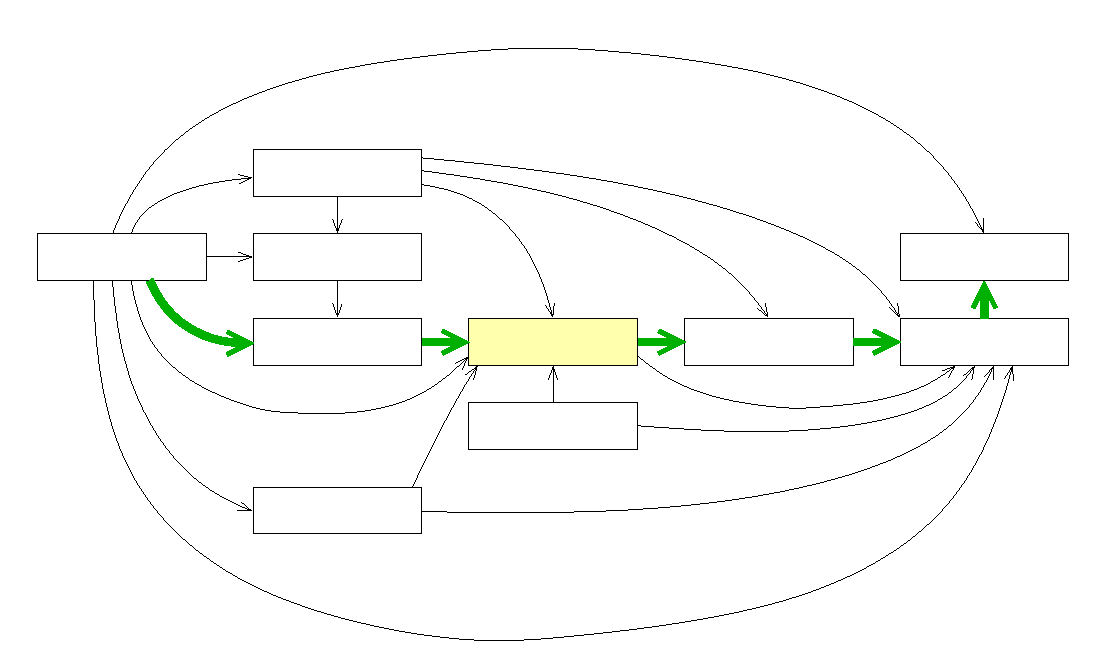
\includegraphics{getdp-struct-formulation}%
\end{picture}%
\setlength{\unitlength}{3947sp}%
%
\begingroup\makeatletter\ifx\SetFigFont\undefined%
\gdef\SetFigFont#1#2#3#4#5{%
  \reset@font\fontsize{#1}{#2pt}%
  \fontfamily{#3}\fontseries{#4}\fontshape{#5}%
  \selectfont}%
\fi\endgroup%
\begin{picture}(8274,4765)(439,-6402)
\put(1126,-3361){\makebox(0,0)[b]{\smash{\SetFigFont{10}{12.0}{\rmdefault}{\mddefault}{\updefault}{\color[rgb]{0,0,0}\code{Group}}%
}}}
\put(2851,-2686){\makebox(0,0)[b]{\smash{\SetFigFont{10}{12.0}{\rmdefault}{\mddefault}{\updefault}{\color[rgb]{0,0,0}\code{Function}}%
}}}
\put(2851,-3361){\makebox(0,0)[b]{\smash{\SetFigFont{10}{12.0}{\rmdefault}{\mddefault}{\updefault}{\color[rgb]{0,0,0}\code{Constraint}}%
}}}
\put(2851,-4036){\makebox(0,0)[b]{\smash{\SetFigFont{10}{12.0}{\rmdefault}{\mddefault}{\updefault}{\color[rgb]{0,0,0}\code{FunctionSpace}}%
}}}
\put(2851,-5386){\makebox(0,0)[b]{\smash{\SetFigFont{10}{12.0}{\rmdefault}{\mddefault}{\updefault}{\color[rgb]{0,0,0}\code{Jacobian}}%
}}}
\put(4576,-4711){\makebox(0,0)[b]{\smash{\SetFigFont{10}{12.0}{\rmdefault}{\mddefault}{\updefault}{\color[rgb]{0,0,0}\code{Integration}}%
}}}
\put(4576,-4036){\makebox(0,0)[b]{\smash{\SetFigFont{10}{12.0}{\rmdefault}{\mddefault}{\updefault}{\color[rgb]{0,0,0}\code{Formulation}}%
}}}
\put(6301,-4036){\makebox(0,0)[b]{\smash{\SetFigFont{10}{12.0}{\rmdefault}{\mddefault}{\updefault}{\color[rgb]{0,0,0}\code{Resolution}}%
}}}
\put(8026,-3361){\makebox(0,0)[b]{\smash{\SetFigFont{10}{12.0}{\rmdefault}{\mddefault}{\updefault}{\color[rgb]{0,0,0}\code{PostOperation}}%
}}}
\put(8026,-4036){\makebox(0,0)[b]{\smash{\SetFigFont{10}{12.0}{\rmdefault}{\mddefault}{\updefault}{\color[rgb]{0,0,0}\code{PostProcessing}}%
}}}
\end{picture}
}}

\chapter{\code{Formulation}: building equations}

\begin{slide}



Example:


\end{slide}

% ---------------------------------------------------------------------------

\background{7\semcm}{4.2\semcm}{\scalebox{0.3}{\begin{picture}(0,0)%
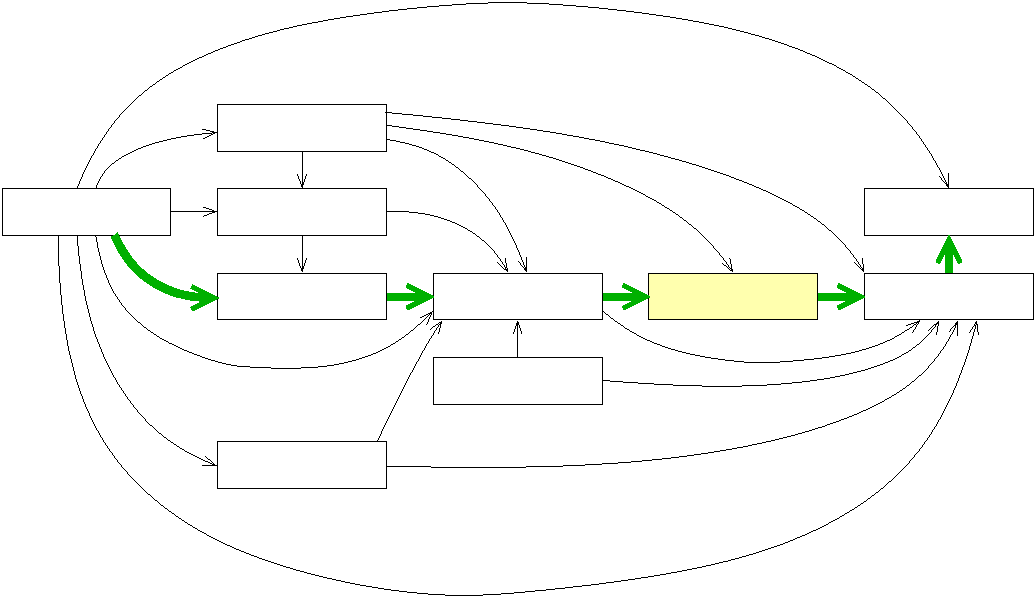
\includegraphics{getdp-struct-resolution}%
\end{picture}%
\setlength{\unitlength}{3947sp}%
%
\begingroup\makeatletter\ifx\SetFigFont\undefined%
\gdef\SetFigFont#1#2#3#4#5{%
  \reset@font\fontsize{#1}{#2pt}%
  \fontfamily{#3}\fontseries{#4}\fontshape{#5}%
  \selectfont}%
\fi\endgroup%
\begin{picture}(8552,4992)(300,-6402)
\put(1126,-3361){\makebox(0,0)[b]{\smash{\SetFigFont{10}{12.0}{\rmdefault}{\mddefault}{\updefault}{\color[rgb]{0,0,0}\code{Group}}%
}}}
\put(2851,-2686){\makebox(0,0)[b]{\smash{\SetFigFont{10}{12.0}{\rmdefault}{\mddefault}{\updefault}{\color[rgb]{0,0,0}\code{Function}}%
}}}
\put(2851,-3361){\makebox(0,0)[b]{\smash{\SetFigFont{10}{12.0}{\rmdefault}{\mddefault}{\updefault}{\color[rgb]{0,0,0}\code{Constraint}}%
}}}
\put(2851,-4036){\makebox(0,0)[b]{\smash{\SetFigFont{10}{12.0}{\rmdefault}{\mddefault}{\updefault}{\color[rgb]{0,0,0}\code{FunctionSpace}}%
}}}
\put(2851,-5386){\makebox(0,0)[b]{\smash{\SetFigFont{10}{12.0}{\rmdefault}{\mddefault}{\updefault}{\color[rgb]{0,0,0}\code{Jacobian}}%
}}}
\put(4576,-4711){\makebox(0,0)[b]{\smash{\SetFigFont{10}{12.0}{\rmdefault}{\mddefault}{\updefault}{\color[rgb]{0,0,0}\code{Integration}}%
}}}
\put(4576,-4036){\makebox(0,0)[b]{\smash{\SetFigFont{10}{12.0}{\rmdefault}{\mddefault}{\updefault}{\color[rgb]{0,0,0}\code{Formulation}}%
}}}
\put(6301,-4036){\makebox(0,0)[b]{\smash{\SetFigFont{10}{12.0}{\rmdefault}{\mddefault}{\updefault}{\color[rgb]{0,0,0}\code{Resolution}}%
}}}
\put(8026,-3361){\makebox(0,0)[b]{\smash{\SetFigFont{10}{12.0}{\rmdefault}{\mddefault}{\updefault}{\color[rgb]{0,0,0}\code{PostOperation}}%
}}}
\put(8026,-4036){\makebox(0,0)[b]{\smash{\SetFigFont{10}{12.0}{\rmdefault}{\mddefault}{\updefault}{\color[rgb]{0,0,0}\code{PostProcessing}}%
}}}
\end{picture}
}}

\chapter{\code{Resolution}: solving systems of equations}

\begin{slide}


Example:


\end{slide}

% ---------------------------------------------------------------------------

\background{7\semcm}{4.2\semcm}{\scalebox{0.3}{\begin{picture}(0,0)%
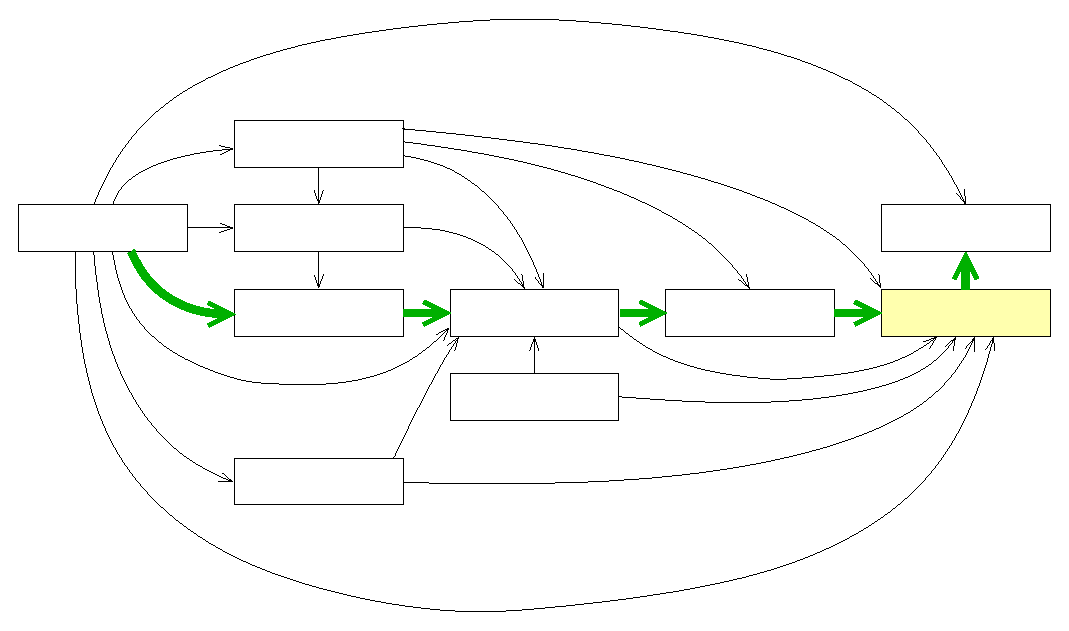
\includegraphics{getdp-struct-postprocessing}%
\end{picture}%
\setlength{\unitlength}{3947sp}%
%
\begingroup\makeatletter\ifx\SetFigFont\undefined%
\gdef\SetFigFont#1#2#3#4#5{%
  \reset@font\fontsize{#1}{#2pt}%
  \fontfamily{#3}\fontseries{#4}\fontshape{#5}%
  \selectfont}%
\fi\endgroup%
\begin{picture}(8274,4765)(439,-6402)
\put(1126,-3361){\makebox(0,0)[b]{\smash{\SetFigFont{10}{12.0}{\rmdefault}{\mddefault}{\updefault}{\color[rgb]{0,0,0}\code{Group}}%
}}}
\put(2851,-2686){\makebox(0,0)[b]{\smash{\SetFigFont{10}{12.0}{\rmdefault}{\mddefault}{\updefault}{\color[rgb]{0,0,0}\code{Function}}%
}}}
\put(2851,-3361){\makebox(0,0)[b]{\smash{\SetFigFont{10}{12.0}{\rmdefault}{\mddefault}{\updefault}{\color[rgb]{0,0,0}\code{Constraint}}%
}}}
\put(2851,-4036){\makebox(0,0)[b]{\smash{\SetFigFont{10}{12.0}{\rmdefault}{\mddefault}{\updefault}{\color[rgb]{0,0,0}\code{FunctionSpace}}%
}}}
\put(2851,-5386){\makebox(0,0)[b]{\smash{\SetFigFont{10}{12.0}{\rmdefault}{\mddefault}{\updefault}{\color[rgb]{0,0,0}\code{Jacobian}}%
}}}
\put(4576,-4711){\makebox(0,0)[b]{\smash{\SetFigFont{10}{12.0}{\rmdefault}{\mddefault}{\updefault}{\color[rgb]{0,0,0}\code{Integration}}%
}}}
\put(4576,-4036){\makebox(0,0)[b]{\smash{\SetFigFont{10}{12.0}{\rmdefault}{\mddefault}{\updefault}{\color[rgb]{0,0,0}\code{Formulation}}%
}}}
\put(6301,-4036){\makebox(0,0)[b]{\smash{\SetFigFont{10}{12.0}{\rmdefault}{\mddefault}{\updefault}{\color[rgb]{0,0,0}\code{Resolution}}%
}}}
\put(8026,-3361){\makebox(0,0)[b]{\smash{\SetFigFont{10}{12.0}{\rmdefault}{\mddefault}{\updefault}{\color[rgb]{0,0,0}\code{PostOperation}}%
}}}
\put(8026,-4036){\makebox(0,0)[b]{\smash{\SetFigFont{10}{12.0}{\rmdefault}{\mddefault}{\updefault}{\color[rgb]{0,0,0}\code{PostProcessing}}%
}}}
\end{picture}
}}

\chapter{\code{PostProcessing}: exploiting computational results}

\begin{slide}



Example:


\end{slide}

% ---------------------------------------------------------------------------

\background{7\semcm}{4.2\semcm}{\scalebox{0.3}{\begin{picture}(0,0)%
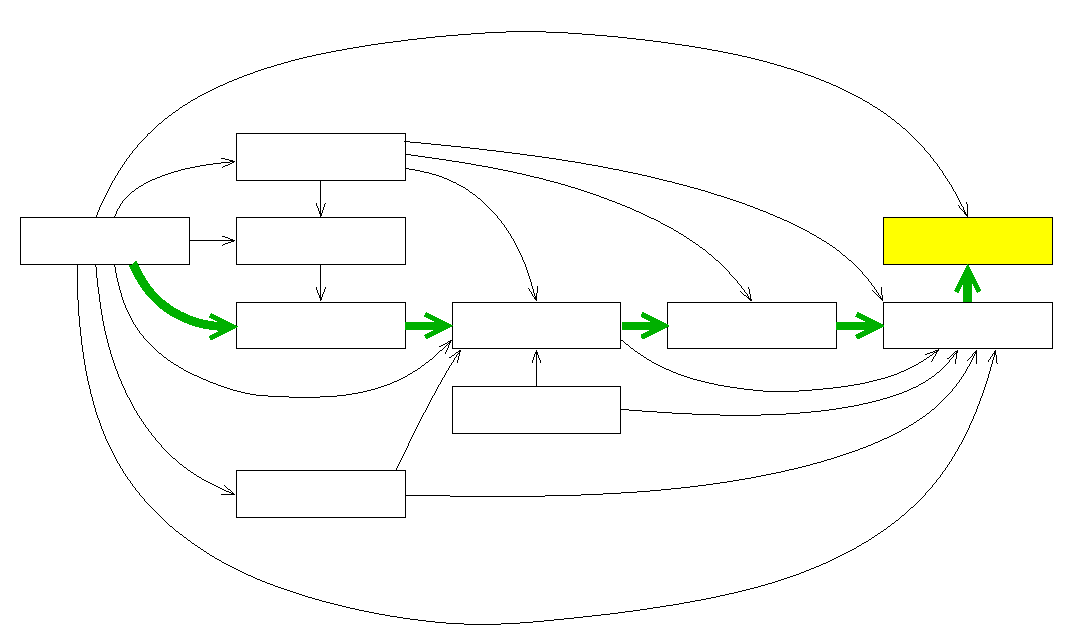
\includegraphics{getdp-struct-postoperation}%
\end{picture}%
\setlength{\unitlength}{3947sp}%
%
\begingroup\makeatletter\ifx\SetFigFont\undefined%
\gdef\SetFigFont#1#2#3#4#5{%
  \reset@font\fontsize{#1}{#2pt}%
  \fontfamily{#3}\fontseries{#4}\fontshape{#5}%
  \selectfont}%
\fi\endgroup%
\begin{picture}(8552,4992)(300,-6402)
\put(1126,-3361){\makebox(0,0)[b]{\smash{\SetFigFont{10}{12.0}{\rmdefault}{\mddefault}{\updefault}{\color[rgb]{0,0,0}\code{Group}}%
}}}
\put(2851,-2686){\makebox(0,0)[b]{\smash{\SetFigFont{10}{12.0}{\rmdefault}{\mddefault}{\updefault}{\color[rgb]{0,0,0}\code{Function}}%
}}}
\put(2851,-3361){\makebox(0,0)[b]{\smash{\SetFigFont{10}{12.0}{\rmdefault}{\mddefault}{\updefault}{\color[rgb]{0,0,0}\code{Constraint}}%
}}}
\put(2851,-4036){\makebox(0,0)[b]{\smash{\SetFigFont{10}{12.0}{\rmdefault}{\mddefault}{\updefault}{\color[rgb]{0,0,0}\code{FunctionSpace}}%
}}}
\put(2851,-5386){\makebox(0,0)[b]{\smash{\SetFigFont{10}{12.0}{\rmdefault}{\mddefault}{\updefault}{\color[rgb]{0,0,0}\code{Jacobian}}%
}}}
\put(4576,-4711){\makebox(0,0)[b]{\smash{\SetFigFont{10}{12.0}{\rmdefault}{\mddefault}{\updefault}{\color[rgb]{0,0,0}\code{Integration}}%
}}}
\put(4576,-4036){\makebox(0,0)[b]{\smash{\SetFigFont{10}{12.0}{\rmdefault}{\mddefault}{\updefault}{\color[rgb]{0,0,0}\code{Formulation}}%
}}}
\put(6301,-4036){\makebox(0,0)[b]{\smash{\SetFigFont{10}{12.0}{\rmdefault}{\mddefault}{\updefault}{\color[rgb]{0,0,0}\code{Resolution}}%
}}}
\put(8026,-3361){\makebox(0,0)[b]{\smash{\SetFigFont{10}{12.0}{\rmdefault}{\mddefault}{\updefault}{\color[rgb]{0,0,0}\code{PostOperation}}%
}}}
\put(8026,-4036){\makebox(0,0)[b]{\smash{\SetFigFont{10}{12.0}{\rmdefault}{\mddefault}{\updefault}{\color[rgb]{0,0,0}\code{PostProcessing}}%
}}}
\end{picture}
}}

\chapter{\code{PostOperation}: exporting results}

\begin{slide}



Example:


\end{slide}

% ---------------------------------------------------------------------------

\background{}{}{}


% $Id: getdp-examples.tex,v 1.2 2001-06-12 16:21:33 geuzaine Exp $

% ---------------------------------------------------------------------------
\part{GetDP examples}
% ---------------------------------------------------------------------------

\chapter{The simplest example: magnetostatics}

\begin{slide}

\mybox{colbox}{\textwidth}{
\begin{equation*}
\Curl{\vec{h}} = \vec{j} ,\quad
\Div{\vec{b}} = 0 \quad\text{and}\quad
\vec{b} = \mu \vec{h} + \mu_0 \vec{h}_m 
\end{equation*}
\begin{equation*}\label{eq:tonti-sta}
\begin{split}
\xymatrix{
 \color{colpos}\phi    \ar@{->}[r]^-{\GradSymb_h}  &
 \vec{h} \ar@{->}[r]^-{\CurlSymb_h} \ar@{<->}[d]^{\mu} &
 \vec{j} \ar@{->}[r]^-{\DivSymb_h}   &
 0 \\
 0       \ar@{<-}[r]^-{\DivSymb_e}&
 \vec{b} \ar@{<-}[r]^-{\CurlSymb_e}&
 \color{colpos}\vec{a} 
}
\end{split}
\end{equation*}
}

\begin{slideitemize}
\item Weak form of Gauss law: 
\begin{equation*}
%\ivol{\Div{\vec{b}}}{\phi'} = 0 \Rightarrow
\ivol{\vec{b}}{\Grad{\phi'}} + \isur{\psca{\vec{n}}{\vec{b}}}{\phi'} 
= 0
\quad \forall\phi'\in\Hone[_0]{\Omega}
\end{equation*}

\item Weak form of Ampere's law:
\begin{equation*}
%\ivol{\Curl{\vec{h}}}{\vec{a}'} = \ivol{\vec{j}}{\vec{a}'} \Rightarrow
\ivol{\vec{h}}{\Curl{\vec{a}'}} + \isur{\pvec{\vec{n}}{\vec{h}}}{\vec{a}'}
= \ivol{\vec{j}}{\vec{a}'} 
\quad \forall\vec{a}'\in\Hcurl[_0]{\Omega}
\end{equation*}

\end{slideitemize}

\end{slide}

\begin{slide}

\mybox{colbox}{\textwidth}{
\begin{center}
\emph{Scalar potential} formulation
\begin{equation*}\label{eq:hs+hr1}
\vec{h} = \vec{h}_s+\vec{h}_r ,\quad\text{with}\quad
\Curl{\vec{h}_s} = \vec{j}     \quad\text{and}\quad
\vec{h}_r = -\Grad{\phi}
\end{equation*}
\end{center}
}

\bigskip
NB: choice of source field $\vec{h}_s$, tretament of multiply connected
$\Omega$, ...

\end{slide}

\begin{slide}

\mybox{colbox}{\textwidth}{
\begin{center}
\emph{Vector potential} formulation
\begin{equation*}\label{eq:hs+hr1}
\vec{b} = \Curl{\vec{a}}
\end{equation*}
\end{center}
}

\bigskip
NB: gauge for $\vec{a}$, ...

\end{slide}

% ---------------------------------------------------------------------------

\background{}{}{}



% ---------------------------------------------------------------------------
\part{Solver integration}
% ---------------------------------------------------------------------------

\chapter{FEM in practice}

\begin{slide}

Four steps

\begin{slideitemize}
\item Geometry
\item Mesh
\item Solver
\item Post-processing
\end{slideitemize}

And most of time is usually not spent on Solver... {\large\color{colwarn}\frownie}

\end{slide}

% ---------------------------------------------------------------------------

\chapter{Batch vs. interactive processing}

\begin{slide}

GetDP has no graphical interface 

Command line

Integration into higher level optimization toolboxes:
\begin{slideitemize}
\item High level: Matlab, Mathematica, shell scripts (Perl, Python, ...),
other programming languages (C, C++, ...)  $\rightarrow$ \emph{system call}
\item Medium level: shell scripts (Perl, Python, ...), other programming
languages (C, C++, ...) $\rightarrow$ \emph{UNIX sockets}
\item Low level: programming languages (C, C++, Fortran) $\rightarrow$
\emph{source code}
\end{slideitemize}


Example: Gmsh

\end{slide}


%% $Id: gmsh.tex,v 1.5 2001-06-13 16:00:29 geuzaine Exp $

\chapter{}

\begin{slide}

\slidepagestyle{reduced}

\begin{center}
\bigtitle{Gmsh --- Geometry, mesh, solver integration
and visualization}\\
\ifthenelse{\boolean{fulltitle}}{
\bigskip\bigskip
\begin{minipage}{0.5\textwidth}\center
\mediumtitle{Christophe Geuzaine}\\
\bigskip
\smalltitle{Dept. of Electrical Engineering}\\
\smalltitle{Montefiore Institute B28, Sart Tilman}\\
\smalltitle{University of Li�ge}\\
\smalltitle{B-4000 Li�ge (BELGIUM)}
\end{minipage}%
\begin{minipage}{0.5\textwidth}\center
\mediumtitle{Jean-Fran�ois Remacle}\\
\bigskip
\smalltitle{Scientific Computation Research Center}\\
\smalltitle{Rensselaer Polytechnic Insitute}\\
\smalltitle{CII 110 8th Street}\\
\smalltitle{Troy, New York 12180-3590 (USA)}
\end{minipage}}
\end{center}

\end{slide}

% ---------------------------------------------------------------------------
\part{Gmsh}
% ---------------------------------------------------------------------------

\chapter{Finite element methods in practice}

\begin{slide}

Four main steps:
\begin{slideitemize}
\item \emph{Geometry}: CAD sofware
\item \emph{Mesh}: structured or unstructed mesh generator
\item \emph{Solver}: GetDP :-)
\item \emph{Post-processing}: various visualization tools (2D and 3D)
\end{slideitemize}

Most of the time spent solving a problem is \emph{not} in the solver step!

\end{slide}

% ---------------------------------------------------------------------------

\background{7\semcm}{4.2\semcm}
           {\scalebox{0.3}{\input{fig/gmsh-geo.tex}}}

\chapter{Geometry description}

\begin{slide}

Constructive:


Parametric (scriptable):



\end{slide}

% ---------------------------------------------------------------------------

\background{7\semcm}{4.2\semcm}
           {\scalebox{0.3}{\input{fig/gmsh-mesh.tex}}}

\chapter{Mesh generation}

\begin{slide}

\begin{slideitemize}
\item \emph{Structured} (transfinite, elliptic, hyperbolic)
\item \emph{Unstructured} (Delaunay triangles/tetrahedra)
\begin{enumerate}
\item 
mesh of a box including the convex polygon/polyhedron resulting from
curves/surfaces discretization
\item
initial mesh by insertion of curves/surfaces nodes by the Bowyer algorithm
\item 
boundary restoration to force presence of all edges/faces
\item 
suppression of undesired triangles/tetrahedra
\item
new node insertions by the Bowyer algorithm until the characteristic size of
each simplex $\leq$ characteristic length field evaluated at the center of
its circumscribed circle/sphere.
\item
mesh post-processing and quality enforcement by node relocation and edge
swapping
\end{enumerate}
\end{slideitemize}

\end{slide}

% ---------------------------------------------------------------------------

\background{7\semcm}{4.2\semcm}
           {\scalebox{0.3}{\input{fig/gmsh-solver.tex}}}

\chapter{Solver integration}

\begin{slide}

\begin{minipage}{0.45\textwidth}
\emph{Batch}:
\begin{slideitemize}
\item Advanced users
\item No graphical overhead
\item Easily scriptable
\end{slideitemize}
$\rightarrow$ for heavy problems
\end{minipage}%
\begin{minipage}{0.1\textwidth}
vs.
\end{minipage}%
\begin{minipage}{0.45\textwidth}
\emph{Interactive}:
\begin{slideitemize}
\item Smoother learning curve
\item Better integration
\item Faster for testing
\end{slideitemize}
$\rightarrow$ for testing/learning
\end{minipage}%

\end{slide}

\begin{slide}

Example: integration of GetDP into higher level toolboxes (visualization,
optimization, etc.):
\begin{slideitemize}
\item \emph{High level}: Commercial applications (Matlab, Mathematica, ...),
shell scripts (bash, Perl, Python, ...), other programming languages (C,
C++, ...) 

$\rightarrow$ \emph{system calls}
\item \emph{Medium level}: Home-grown applications (Gmsh, ...), shell scripts
(Perl, Python, ...), other programming languages (C, C++, ...) 

$\rightarrow$ \emph{sockets}
\item \emph{Low level}: programming languages (C, C++, ...) 

$\rightarrow$ \emph{source code}
\end{slideitemize}

\end{slide}

% ---------------------------------------------------------------------------

\background{7\semcm}{4.2\semcm}
           {\scalebox{0.3}{\input{fig/gmsh-postpro.tex}}}

\chapter{Post-processing}

\begin{slide}

Scriptable:

Modular:


\end{slide}

% ---------------------------------------------------------------------------





% ---------------------------------------------------------------------------
\part{Collaboration}
% ---------------------------------------------------------------------------

\chapter{Possible collaboration topics}

\begin{slide}

\begin{slideitemize}
\item Error estimation
\item Optimization
\end{slideitemize}

\end{slide}

% ---------------------------------------------------------------------------
\part{Conclusion}
% ---------------------------------------------------------------------------

\chapter{Conclusions}

\begin{slide}

Open software: input text files, no physics in code, free.

Current aids: mailing lists, documentation

Interactive use through Gmsh


\end{slide}


\end{document}

